\documentclass[a4paper, 12pt]{book}

% ===== PACCHETTI NECESSARI ===== %
\usepackage[margin=2.5cm]{geometry}
\usepackage[italian]{babel}
%\usepackage{wrapfig}
\usepackage{graphicx}   % per inserire immagini
\usepackage{ulem} 
\usepackage{caption}    % per le didascalie
\usepackage{subcaption} % per sottodidascalie
\usepackage{hyperref}
\usepackage{tikz}
\usetikzlibrary{positioning, shapes, arrows.meta}
\usepackage[T1]{fontenc}
\usetikzlibrary{calc}
\usepackage{float}
\usepackage{amsmath}
\setlength{\parindent}{0pt}
\usepackage{parskip}
\usepackage{soul}
\usepackage{xcolor}
\sethlcolor{yellow}
\usepackage{array}\usepackage[most]{tcolorbox}
\usepackage{booktabs}
\usepackage{tikz}
\usetikzlibrary{positioning}
\usepackage{longtable}
\usepackage{array}
\usepackage{fancyhdr}
\setlength{\headheight}{15pt}
\pagestyle{fancy}
\fancyhf{} % pulisce header e footer
\fancyhead[R]{\thepage} % numero pagina a destra nell'header
\renewcommand{\headrulewidth}{0pt} % (opzionale) elimina la riga orizzontale sotto l'header
\fancypagestyle{plain}{%
  \fancyhf{} % pulisce header e footer
  \fancyhead[R]{\thepage} % numero sempre in alto a destra
  \renewcommand{\headrulewidth}{0pt} % opzionale: niente linea
}
\setcounter{tocdepth}{3}


% ===== LISTA COMANDI =====
%------COMANDO SOTTOLINEA-------%
\newcommand{\sottolinea}[2]{%
  {\setulcolor{#1}\ul{#2}}%
}

%------COMANDO DEFINIZIONE-------%
\newcommand{\definizione}[2]{%
  \vspace{15pt}%
  \begin{tcolorbox}[
    colback=cyan!5!white,
    colframe=blue!50!black,
    title=\textbf{Definizione - #1}, % titolo della definizione
    coltitle=white,
    fonttitle=\bfseries,
    arc=3mm,
    boxrule=0.5pt,
    enhanced,
    breakable
  ]
  #2 % testo della definizione
  \end{tcolorbox}
  \vspace{15pt}%
}

%------COMANDO TESTO ESERCIZIO-------%
\newcommand{\esercizioTesto}[2]{%
  \vspace{15pt}%
  \begin{tcolorbox}[
    colback=green!5!white,
    colframe=green!60!black,
    title=\textbf{Esercizio - #1}, % titolo della definizione
    coltitle=white,
    colbacktitle=green!40!black, % PARAMETRO per il frame del titolo
    fonttitle=\bfseries,
    arc=3mm,
    boxrule=0.5pt,
    enhanced,
    breakable
  ]
  #2 % testo della definizione
  \end{tcolorbox}
  \vspace{15pt}%
}

%------comando ESEMPIO-------%
\newcommand{\esempio}[2]{%
  \begin{center}
    \textbf{#1}\par
    #2
  \end{center}
}




\title{\textbf{Basi di dati - primo semestre}\\uniVR - Dipartimento di Informatica}
\author{Mattia Nicolis \and Matteo Drago}
\date{A.A. 2025-26}

\begin{document}

  \maketitle

  \tableofcontents
  \markboth{}{}

  %-------MODULO DI TEORIA------------------------------------
  %-------Prof: Alberto Belussi-------------------------------
  %-------Lez: Martedì (10:30-12:30) [Aula A - Cav.1]----------
  %-------Lez: Venerdì (11:30-13:30) [Aula A - Cav.1]----------

  \chapter*{Introduzione}
  \addcontentsline{toc}{chapter}{Introduzione}

  \section*{Storia delle DBMS}
  \addcontentsline{toc}{section}{Storia delle DBMS}


  La nascita dei sistemi per la gestione di basi di dati ha visto due momenti principali:
  \begin{description}   % Ambiente description, [parola] in grassetto 
    \item \textbf{anni '60}: sviluppo di applicazioni negli \textbf{ambienti di ricerca scientifica}
    \item \textbf{anni '70}: sviluppo di applicazioni informatiche in \textbf{ambito gestionale}
  \end{description}

  Si trattava di semplici dispositivi in cui gli \uline{algoritmi} di elaborazione \uline{erano semplici} e \uline{grandi quantità di dati} erano \uline{\textbf{condivisi}} da più applicazioni.
  
  Queste caratteristiche erano specifiche per l'ambiente in cui erano state introdotte ovvero il \textbf{sistema informativo}.

  \definizione{Sistema informativo}{    L'insieme delle attività umane e dei dispositivi di memorizzazione ed elaborazione che organizza e gestisce l'informazione di interesse per una organizzazione di dimensioni qualsiasi.
  }


  Il sistema informativo è costituito da \textit{dati} e \textit{informazioni}:
  \begin{itemize}
    \item \textbf{dato}: elemento di conoscenza di base costituito da simboli che devono essere elaborati
    \item \textbf{informazione}: interpretazione dei dati che permette di ottenere conoscenza più o meno esatta di fatti e situazioni
  \end{itemize}
  
  Lo studio del sistema informativo avviene attraverso i \textbf{diagrammi di flusso}, questi permettono di svolgere diverse operazioni tra cui: 
  \begin{itemize}
    \item definizione archivi dati e delle sorgenti di dati
    \item definizione degli utenti
    \item definizione di procedure e processi
    \item definizione dei flussi dati
  \end{itemize}


  \clearpage
  \textbf{\large Come si è arrivati allo sviluppo dei DBMS?}

  Negli anni '70 i programmi comunicavano direttamente con i dati contenuti nel file system. 
  
  Era un'operazione scomoda in quanto l’accesso ai dati su file era scarso (\textbf{struttura ad accesso sequenziale}), c'era ridondanza nei dati (\textbf{duplicazioni dello stesso dato su più file}), c'era inconsistenza dovuta ad aggiornamenti parziali e la progettazione dei dati era replicata per ogni programma.

  Negli anni '80 la soluzione che venne proposta fu quella di inserire un \textbf{DBMS} (Data Base Management System) tra il \textbf{file system} e le \textbf{applicazioni}.

  \begin{figure}[h]
    \centering

    \begin{subfigure}[b]{0.45\textwidth}
      \centering
      \includegraphics[width=\textwidth, height=3.8cm]{images/fileSystem.png}
      \caption{Solo file system}
    \end{subfigure}
    \hfill
    \begin{subfigure}[b]{0.45\textwidth}
      \centering
      
\includegraphics[width=\textwidth, height=3.8cm]{images/DBMS.png}
      \caption{File system + base di dati}
    \end{subfigure}

  \caption{Prima e dopo l'innovazione}
  \end{figure}

  \definizione{Base di dati}{Una collezione di dati utilizzati per rappresentare con tecnologia informatica le informazioni di interesse per un sistema informativo.
  }

  \definizione{DBMS}{Sistema che gestisce su memoria secondaria collezioni di dati \textbf{grandi}, \textbf{condivise} e \textbf{persistenti}, assicurandone l'\textbf{affidabilità} la \textbf{privatezza} e l'\textbf{accesso efficiente}.
  }

  Questo nuovo approccio ha portato numerosi vantaggi:
  \begin{itemize}
    \item \textbf{maggiore astrazione} e più potenza espressiva per descrivere le proprietà del dato.
    \hl{All'interno del \textbf{DMBS} i dati vengono interpretati come oggetti, ovvero istanze di classi o righe di tabelle}.
    
    Prima erano interpretati come blocchi o pagine di memoria secondaria (sequenze di byte)

    \item \textbf{operazioni di accesso ai dati più complesse} basate su un \uline{linguaggio di interrogazione} (SELECT FROM WHERE) anzichè attraverso operazioni di READ/WRITE
    \item \textbf{migliorata l'interazione uomo-informazione:} 
    \begin{itemize}
      \item linguaggio per la definizione dei dati (Data Definition Language - DDL)
      \item linguaggio per l’interrogazione e aggiornamento dei dati (Data Manipulation Language – DML): 
      \begin{itemize}
        \item linguaggio di interrogazione: estrae informazioni da una base di dati (esempio: SQL, algebra relazionale)
        \item linguaggio di manipolazione: popola la base di dati, modifica il suo contenuto con aggiunte, cancellazioni e variazioni sui dati (es. SQL)
      \end{itemize}
    \end{itemize}
  \end{itemize}

  
  \definizione{DBMS: modello dei dati}{ È l’insieme dei costrutti forniti dal DBMS per descrivere la struttura e le proprietà dell’informazione contenuta in una base di dati.
  
  \vspace{1mm}
  
  I costrutti permettono di definire le strutture dati che conterrano le informazioni e specificare le proprietà che dovranno soddisfare le istanze.
  }


  Nel \uline{passato} esistevano modelli come quello \uline{reticolare} o quello \uline{gerarchico}.

  Attualmente si parla di modello relazionale, ad oggetti, object-relational (SQL99 o SQL3), basato sui documenti(JSON) o NoSQL.

  \definizione{Schema di una base di dati}{È la descrizione della struttura e delle proprietà di una specifica base di dati fatta utilizzando i costrutti del modello dei dati (lo schema di una base di dati è invariante nel tempo).
  }

  \definizione{Istanza di una base di dati}{È costituita dai valori effettivi che in un certo istante popolano le strutture dati della base di dati (l’istanza di una base di dati varia nel tempo).}


  \begin{figure}[H] %% Messo H anzichè h in questo modo il testo sotto non passa sopra la foto in quanto troppo grande
      \centering
      \includegraphics[width=0.7\textwidth]{images/modelloSchemaIstanza.png}
      \caption{Distinzione tra modello, schema e istanza}
  \end{figure}



  \section*{Architettura di un DBMS}
  \addcontentsline{toc}{section}{Architettura di un DBMS}

  \begin{itemize}
    \item \textbf{schema logico}: è la rappresentazione della struttura e delle proprietà della base di dati definita attraverso i costrutti del modello dei dati del DBMS
    \item \textbf{schema interno}: è la rappresentazione della base di dati per mezzo delle strutture fisiche di memorizzazione (file dati, file indice, ecc…)
    \item \textbf{schema esterno}: descrive una porzione dello schema logico di interesse per uno specifico utente o applicazione (attraverso viste sullo schema logico)
  \end{itemize}

  
  La caratteristica fondamentale di queste strutture è l'\textbf{indipendenza}.
  \begin{description}
    \item \textbf{indipendenza fisica}: lo \uline{schema logico} della base di dati \uline{è completamente indipendente dallo schema interno}. 
    Ne consegue che le variazioni delle strutture fisiche non impattano sullo schema logico e quindi sulle applicazioni.
    \item \textbf{indipendenza logica}: gli \uline{schemi esterni} della base di dati \uline{sono indipendendi dallo schema logico}. 
    Ne consegue che le variazioni dello schema logico (purchè non vengano rimossi dati) non impattano sugli schemi esterni e quindi sulle applicazioni (eventualmente è necessario solo ridefinire l'espressione di derivazione).
  \end{description}
    

  \chapter*{Progettazione di una base di dati}
  \addcontentsline{toc}{chapter}{Progettazione di una base di dati}

  La progettazione di una base di dati costituisce solo una delle componenti del processo di sviluppo di un sistema informativo e va, quindi, inquadrata in un contesto più ampio: il \textbf{ciclo di vita} dei sistemi infoormativi.

  Il \textit{ciclo di vita} di un sistema informativo comprende:
  \begin{enumerate}
    \item \textbf{studio della fattibilità}: \hl{definisce (nel modo più preciso possibile) i \textit{costi} delle varie alternative} possibili e \hl{stabilisce le \textit{priorità} di realizzazione} delle varie componenti del sistema
    \item \textbf{raccolta e analisi dei requesiti}: individua e studia le proprietà e le funzionalità del sistema, producendo una descrizioe completa, ma informale, dei dati coinvolti e delle operazione su di essi.
    \item \textbf{progettazione}: si divide in
    \begin{itemize}
      \item \textit{progettazione dei dati}: descrive la struttura e l'organizzazione dei dati
      \item \textit{progettazione delle apllicazioni}: descrive in modo formale le caratteristiche dei programmi applicativi
    \end{itemize}

    Le due attività sono complememtari e possono procedere in parallelo o in cascata.

    \item \textbf{implementazione}: realizza il sistema informativo secondo la struttura e le caratteristich definite nella fase di progettazione.
    
    Viene costruita e popolata la base di dati e viene prodotto il codice dei programmi.

    \item \textbf{validazione e collaudo}: verifica il corretto funzionamento e la qualità del sistema informativo.
    
    La sperimentazione deve prevedere, per quanto possibile, tutte le confizioni operative.

    \item \textbf{funzionamento}: entra in funzione il sistema informativo ed esegue i compiti per i quali era stato originariamente progettato.
    
    Se non si verificano malfunionamenti o revisioni delle funzionalità del sistema, questa attività richiede solo operazioni di gestione e manutenzione.
  \end{enumerate}

  \begin{figure}[H]
    \centering
    \includegraphics[width=0.2\textwidth, keepaspectratio]{images/cicloVita.jpeg}
    \caption{ciclo di vita}
  \end{figure}

  \section*{Metodologie di progettazione dei dati}
  \addcontentsline{toc}{section}{Metodologie di progettazione dei dati}
  Una \textbf{metologia di progettazione} è costituita da:
  \begin{itemize}
    \item \textbf{decomposizone} dell'intera attività di proegetto in passi sucessivi indipendeneti tra loro
    \item \textbf{insieme di strategie} da seguire nei vari passi e alcuni \textit{criteri} per la scelta in caso di alternative
    \item \textbf{modelli di riferimento} per descrivere i dati di ingresso e uscita delle varie fasi
  \end{itemize}

  Le \textit{proprietà} che una buona metologia deve avere sono:
  \begin{itemize}
    \item \textbf{generale} rispetto alle applicazioni e ai sistemi in gioco (essere inipendendete dal problema studiato e dagli strumenti utilizzati)
    \item \textbf{prodotto di qualità} in termini di \textit{correttezza}, \textit{completezza} ed \textit{efficienza} delle risorse impiegate
    \item \textbf{facile da usare} nelle strategie e neo modelli di riferimento
  \end{itemize}

  Nell'ambito delle basi di dati, si è consolidata negli anni una metodologia di proegetto che ha dato prova di soddisfare pienamente le proprietà descritte.

  Tale metodologia è articolata in tre fasi principali da effettuare a cascata:
  \begin{itemize}
    \item \textbf{progettazione concettuale}: rappresenta le specifiche informali della realtà di interesse in termini di una \hl{descrizione formale e completa}, ma \textit{indipendente} dai criteri di rappresentazione utilizzati nei sistemi di gestione di basi di dati (\textit{schema concettuale}) 
    \item \textbf{progettazione logica}: traduce lo schema concettuale, definito nella fase precedente, in termini del modello di rappresentazione dei dati adottato dal sistema di gestione di base di dati a disposizione (\textit{schema logico}).
    
    Il modello logico, ci consente di descrivere i dati secondo una rappresentazione ancora indipendente da dettagli fisici, ma concreta perchè diposnibile nei sistemi di gestione di base di dati.
    
    \item \textbf{progettazione fisica}: viene completato lo schema logico con la specifica dei parametri fisici di memorizzazione dei dati (\textit{schema fisico})
  \end{itemize}

  \begin{figure}[H]
    \centering
    \includegraphics[width=0.2\textwidth, keepaspectratio]{images/progettazioneACascata.jpeg}
    \caption{progettazione a cascata}
  \end{figure}

  \section*{Modello entità-relazione}
  \addcontentsline{toc}{section}{Modello entità-relazione}
  Il \textbf{modello entità-relazione} è un \textit{modello concettuale} di dati e fornisce una serie di strutture (\textit{costrutti}), atte a descrivere la realtà di interesse in una maniera facile da comprendere e che prescinde dai criteri di organizzazione dei dati nei calcolatori.

  Questi costrutti vengono utilizzati per definire \textit{schemi} che descrivono l'organizzazione e la struttura delle \textit{occorenze} dei dati, dei valori assunti dai dati al variare del tempo.

  \subsection*{Entità}
  \addcontentsline{toc}{subsection}{Entità}
  Un'\textbf{entità E} \hl{rappresenta una classe di oggetti} che hanno proprietà comuni ed esistenza "autonoma" ai fini dell'applicazione di interesse (\textit{Città}, \textit{Dipartimento}, \textit{impiegato}, \textit{Acquiesto}, \textit{Vendita} ecc.).

  Un'occorenza di un'entità è un oggetto della classe che l'entità rappresenta (città di Roma, Milano e Palermo sono occorenze dell'entità \textit{Città}).

  Un'occorenza di entità ha un'esistenza indipendente dalle proprietà a esso associate.

  In uno schema, ogni ha un nome che la identifica univocamente e viene rappresentata graficamente mediante un rettangono con il nome dell'intetà all'interno.

  \begin{figure}[H]
    \centering
    \includegraphics[width=0.5\textwidth, keepaspectratio]{images/entità.jpeg}
    \caption{entità}
  \end{figure}

  \subsubsection*{Identificatori delle entitità}
  \addcontentsline{toc}{subsubsection}{Identificatori delle entitità}
  Un'\textbf{identificatore} di un'entità E è un insieme di attributi di E che \hl{consente di identificare univocamente ciascuna occorrenza di E}.

  In molti casi, uno o più attributi di un'entità sono sufficienti a individuare un identificatore: si parla in questo caso di \textbf{identificatore interno}.

  \esercizioTesto{Esempio di identificare interno}{Un identificatore interno per l'entità \textit{Automobile} con attributi \textit{Targa}, \textit{Modello}, \textit{Colore} e \textit{Anno di immatricolazione} è costituito dall'attributo \textit{Targa}, in quanto ogni automobile ha una targa univoca e non posso esistere due automobili con la stessa targa.
    \begin{figure}[H]
      \centering
      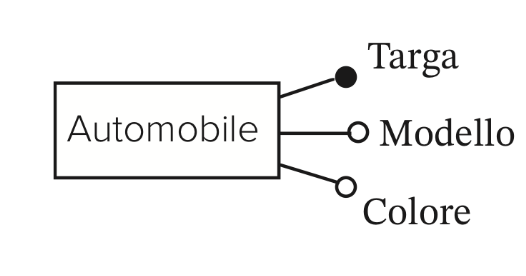
\includegraphics[width=0.5\textwidth, keepaspectratio]{images/identificatoreInterno.png}
      \caption{identificatore interno}
    \end{figure}
  }

  Nei casi in cui l'identificazione di un'entità è ottenuta utilizzando attributi di altre entità, si parla di \textbf{identificatore esterno}.

  \esercizioTesto{Esempio di identificatore esterno}{Nell'entità \textit{Studente}, sembrerebbe a prima vista che l'attributo \textit{Matricola} possa essere un identificatore interno, in quanto ogni studente ha una matricola univoca.
    
  Tuttavia, se si considera che la matricola viene assegnata da un'università, si può notare che due studenti iscritti a due università diverse potrebbero avere la stessa matricola.
    
  In questo caso, un identificatore esterno per l'entità \textit{Studente} potrebbe essere costituito dagli attributi \textit{Matricola} e \textit{Università}, in quanto la combinazione di questi due attributi consente di identificare univocamente ciascuno studente.
    
  \begin{figure}[H]
    \centering
    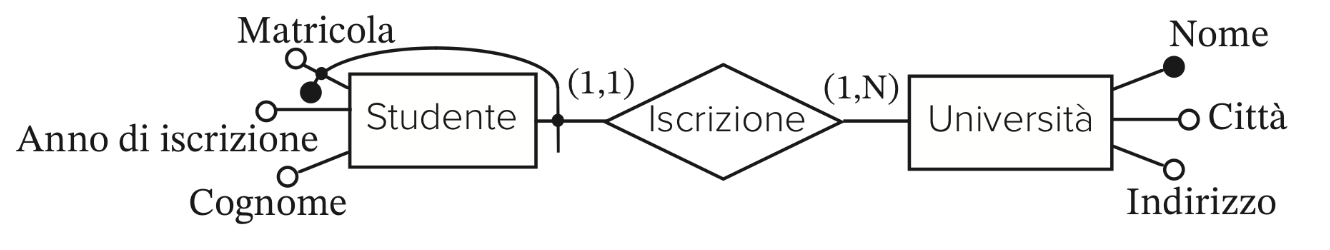
\includegraphics[width=0.5\textwidth, keepaspectratio]{images/identificatoreEsterno.png}
    \caption{identificatore esterno}
  \end{figure}
  }

  \subsection*{Relazioni (associazioni)}
  \addcontentsline{toc}{subsection}{Relazioni (associazioni)}
  Una \textbf{relazione R} \hl{rappresneta un legame logico tra due o più entità} (\textit{Residenza} è una relazione che può sussistere tra le entità \textit{Città} e \textit{Impiegato}).

  Un'occorenza di relazione è un'ennupla costituita da occorenze di entità, una per ciascuna delle entità coinvolte.

  In uno schema E-R, ogni relazione ha un nome che identifica univocamente e viene rappresentata graficamente mediante un rombo con il nome delle realzione al'interno e da linee che connettono la relazione con ciascuna delle sue componenti.

  L'insieme delle occorrenze di una relazione del modello E-R è, una relazione matematica tra le occorenze delle entità coinvolte, ossia, un sottoinsieme del loro prodotto cartesiano.

  Questo significa che tra le occorenze di una relazione del modello E-E non ci possono essere ennuple ripeute.

  \begin{figure}[h]
    \centering

    \begin{subfigure}[b]{0.45\textwidth}
      \centering
      \includegraphics[width=\textwidth, height=3.8cm]{images/relazioniEntità.jpeg}
      \caption{relazioni tra entità}
    \end{subfigure}
    \hfill
    \begin{subfigure}[b]{0.45\textwidth}
      \centering
      \includegraphics[width=\textwidth, height=3.8cm]{images/relazioniRicorsive.jpeg}
      \caption{relazione ricorsiva}
    \end{subfigure}
  \end{figure}

  E' anche possibile avere \textit{relazioni ricorsive}: relazioni tra un'entità e se stessa.

  E' possibile, infine, avere \textit{relazioni n-arie} che coinvolgono più di due entità.

  \begin{figure}[H]
    \centering
    \includegraphics[width=0.5\textwidth, keepaspectratio]{images/relazioneTernaria.jpeg}
    \caption{relazione ternaria}
  \end{figure}

  

  \subsubsection*{Relazioni ternarie}
  \addcontentsline{toc}{subsubsection}{Relazioni ternarie}
  La relazione ternaria è un particolare tipo di relazione che viene utilizzata quando:
  \begin{itemize}
    \item un'istanza del concetto per esistere nel sistema informativo (e quindi nella base di dati) richiede sempre la presenza di tre istanze di entità (una per ogni entità coinvolta nella relazione).
    \item Non esistono eccezioni al punto precedente.
    \item Non esistono situazioni nelle quali la terna di entità debba essere rappresentata più volte.
  \end{itemize}

  \sottolinea{red}{Esempio di uso corretto:}\par
  Vogliamo rappresentare il fatto che un prodotto venga fornito ad un dipartimento da un fornitore. Ogni dipartimento può scegliere quali prodotti ordinare dai fornitori selezionando un sottoinsieme dei profotto forniti dal fornitore. Ogni fornitore vende a più dipartimenti prodotto diversi. Ogni prodotto viene venduto da più fornitori.

  \subsubsection*{Cardinalità delle relazioni}
  \addcontentsline{toc}{subsubsection}{Cardinalità delle relazioni}
  La \textbf{cardinalità} viene specificata per ciascuna partecipazione di entità a una relazione ed esprime il numero (minimo, massimo) di occorenze di un'entità che possono essere associate ad una occorrenza di un'altra entità attraverso la relazione.

  \begin{figure}[H]
    \centering
    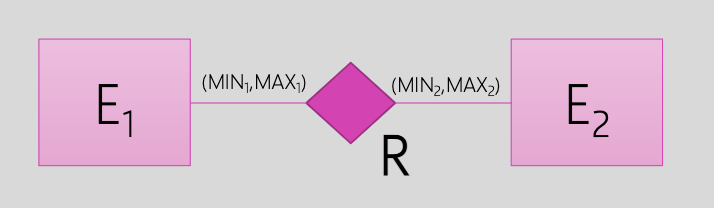
\includegraphics[width=0.5\textwidth, keepaspectratio]{images/cardinalità-relazioni.png}
    \caption{cardinalità delle relazioni}
  \end{figure}

  In linea di principio la cardinalità può essere qualsiasi coppia di numeri naturali (incluso 0 e $\infty$), con l'unico vincolo che la cardinalità minima deve essere minore o uguale della cardinalità massima.

  In realtà, nella maggior parte dei casi, le \hl{\textit{cardinalità minime} sono 0 o 1} e le \hl{\textit{cardinalità massime} sono 1 o N}.

  \begin{figure}[H]
    \centering
    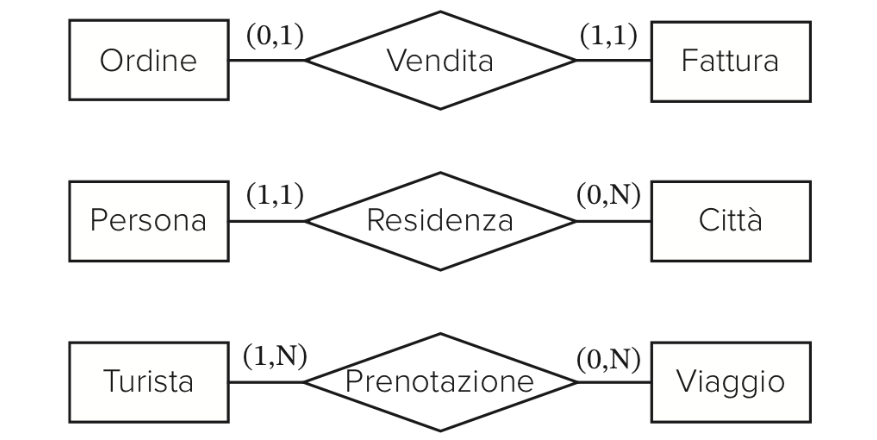
\includegraphics[width=0.5\textwidth, keepaspectratio]{images/esempiCardinalità.png}
    \caption{esempi di cardinalità}
  \end{figure}

  \begin{description}
    \item [cardinalità minima 0 o 1]: significa che la partecipazione di un'entità ad una relazione può essere \textit{facoltativa} (0) o \textit{obbligatoria} (1)
    \item [cardinalità massima 1 o N]: significa che la partecipazione di un'entità ad una relazione può essere \textit{singola} (1) o \textit{multipla} (N) 
  \end{description}

  \definizione{N.B.}{Una relazione R può partecipare ad un identificatore esterno di un'entità E solo se la tale entità partecipa alla relazione con vincolo di cardinalità (1,1) o R è la sola proprietà che partecipa all'identificatore esterno di E.
  \begin{center}
    \begin{minipage}[b]{0.45\textwidth}
      \centering
      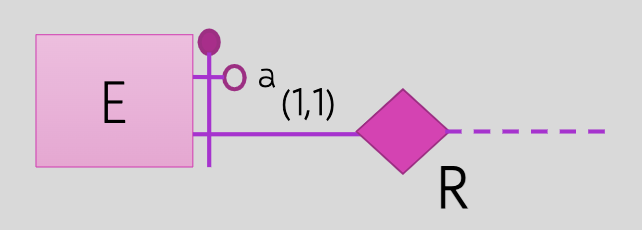
\includegraphics[width=\textwidth, height=3.8cm]{images/esempio1.png}\\
      \textbf{(a)} caso 1
    \end{minipage}
    \hfill
    \begin{minipage}[b]{0.45\textwidth}
      \centering
      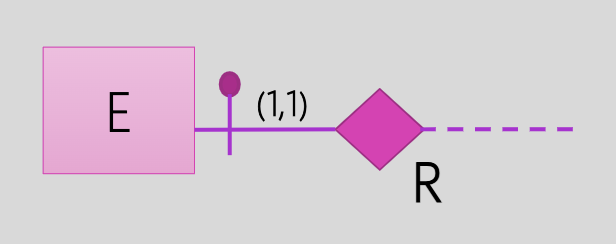
\includegraphics[width=\textwidth, height=3.8cm]{images/esempio2.png}\\
      \textbf{(b)} caso 2
    \end{minipage}
  \end{center}
  }
  
  \subsection*{Attributi}
  \addcontentsline{toc}{subsection}{Attributi}
  Un \textbf{attributo} \hl{descrive le proprietà elementari di un'entità (o relazione)} (\textit{Cognome}, \textit{Stipendio} ed \textit{Età} sono possibili attributi dell'enità \textit{Impiegato}).

  Un attributo associa a ciascuna occorrenza di entità (o di relazione) un valore appartenente a un insieme (\textit{dominio}), che contiene i valori ammissibili per l'attributo.

  I domini non vengono riportati nello schema, ma sono generalmente nella documentazione associata.

  Può risultare comodo raggruppare attributi della medesima entità (o relazione) che presentano affinità nel loro significto o uso (\textit{attributo composto}), ad esempio \textit{Via}, \textit{Numero civico} e \textit{CAP} possono formare l'attributo composto \textit{Indirrizzo} dell'entità \textit{Persona}.

  \begin{figure}[H]
    \centering
    \includegraphics[width=0.5\textwidth, keepaspectratio]{images/attributoComposto.jpeg}
    \caption{attributo composto}
  \end{figure}

  Un esempio completo di \textbf{modello E-R}, può essere il seguente:
  \begin{figure}[H]
    \centering
    \includegraphics[width=0.5\textwidth, keepaspectratio]{images/modelloE-R.jpeg}
    \caption{modello E-R completo}
  \end{figure}

  \subsubsection*{Cardinalità degli attributi}
  \addcontentsline{toc}{subsubsection}{Cardinalità degli attributi}
  Possono essere specificate specificate per gli attributi di un'entità (o relazione) le \textbf{cardinalità} che esprimono il numero (minimo, massimo) di valori che l'attributo può assumere per ciascuna occorrenza dell'entità (o relazione).
  
  Nella maggior parte dei casi, le cardinalità di un attributo è pari a (1,1) e viene omessa nella rappresentazione grafica: in questi casi l'attributo rappresenta sostenzialmente una funzione che associa a ogni occorenza dell'entità (o relazione) un unico valore del dominio dell'attributo.

  Il valore per un certo attributo può essere \textit{nullo} (cardinalità minima 0) o possono essere associati più valori (cardinalità massima N): nel primo caso si dice che la partecipazione dell'attributo è \textbf{opzionale}, nel secondo caso si dice che la partecipazione è \textbf{obblogatoria}.

  \begin{figure}[H]
    \centering
    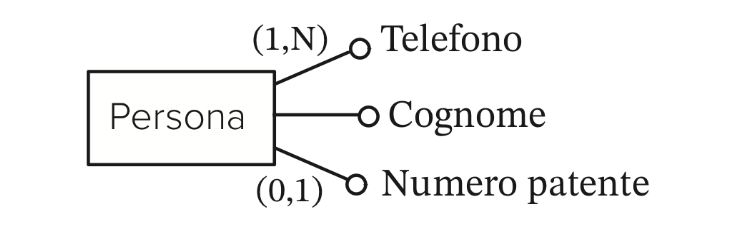
\includegraphics[width=0.5\textwidth, keepaspectratio]{images/cardinalità-attributi.png}
    \caption{cardinalità degli attributi}
  \end{figure}

  Un attributo con cardinalità massima N viene detto \textbf{attributo multivalore} e devono essere utilizzati con cautela, perchè rappresentano situazioni che possono essere modellate, in alcune occasioni, in modo più appropriato mediante l'introduzione di nuove entità e relazioni.


  \section*{Generalizzazione}
  \addcontentsline{toc}{section}{Generalizzazione}
  La \textbf{generalizzazione} è un meccanismo di astrazione che consente di raggruppare entità che condividono alcune proprietà comuni in una entità più generale.

  Rappresentano legami logici tra un'entità \textit{E} (entità genitore) e una o più entità \textit{E1, E2, ..., En} (entità figlie), dove ciascuna entità figlia $E_i$ è una specializzazione dell'entità genitore \textit{E}.

  \esercizioTesto{Esempio di generelizzazione}{L'entità \textit{Persona} è una generelizzazione delle entità \textit{Uomo} e \textit{Donna}, in quanto entrambe le entità figlie condividono alcune proprietà comuni con l'entità genitore, come il nome, il cognome e la data di nascita.
  
  \begin{figure}[H]
    \centering
    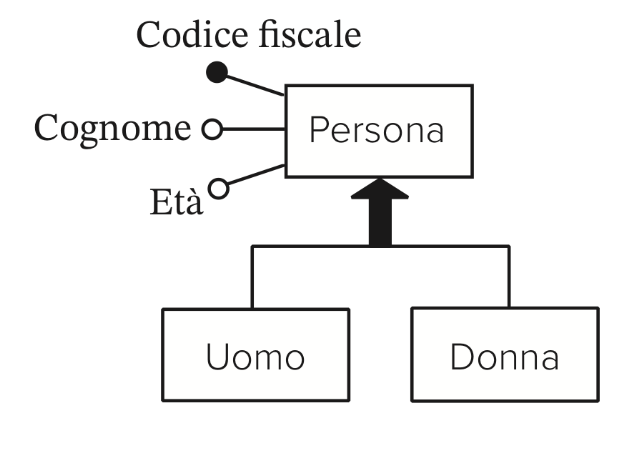
\includegraphics[width=0.5\textwidth, keepaspectratio]{images/generalizzazione.png}
    \caption{generalizzazione}
  \end{figure}
  }

  Le generalizzazioni vengono rappresentate graficamente mediante delle frecce che collegano l'entità genitore alle entità figlie.

  Le generalizzazioni possono essere di due tipi:
  \begin{itemize}
    \item \textbf{totale}: ogni occorrenza dell'entità genitore deve essere anche un'occorrenza di una delle entità figlie (altrimenti è \textbf{parziale})
    \item \textbf{esclusiva}: ogni occorrenza dell'entità genitore può essere anche un'occorrenza di una sola delle entità figlie (altrimenti è \textbf{sovrapposta})
  \end{itemize}

  La generelizzazione tra \textit{Persona}, \textit{Uomo} e \textit{Donna} è totale ed esclusiva, in quanto ogni persona deve essere o un uomo o una donna e non può essere entrambe le cose.


  \chapter*{Esercizi}
  \addcontentsline{toc}{chapter}{Esercizi}

  \section*{Progettazione concettuale}
  \addcontentsline{toc}{section}{Progettazione concettuale}

  \subsection*{Esercizio 1 - guidato}
  \addcontentsline{toc}{subsection}{Esercizio 1 - guidato}


  \esercizioTesto{Progettazione concettuale}{Progettare una base di dati che contenga le informazioni che descrivono la carriera di uno studente del corso di laurea triennale in informatica dal momento dell’immatricolazione fino alla laurea. In particolare, il sistema registra tutti gli esami sostenuti dagli studenti durante la loro carriera. \\
  Per ogni studente si memorizzano: il nome, il cognome, la data di nascita, la matricola (univoca), la data di immatricolazione e la data di laurea. Per ogni insegnamento erogato si memorizzano: la denominazione, l’anno accademico di erogazione, l'anno di corso (I, II o III) e il docente. \\
  Si vuole tener traccia nella base di dati per ogni studente:
  \begin{itemize}
    \item degli insegnamenti frequentati indicando la percentuale di presenza ($>$ 0) di uno studente alle lezioni e
    \item degli esami sostenuti indicando la data dell’esame e il voto finale.
  \end{itemize}
  Si vuole inoltre \uline{poter calcolare} quanti studenti hanno frequentato un insegnamento.
  }

  Soluzione iniziale fornita dal prof (errata):

  \begin{figure}[h]
      \centering
      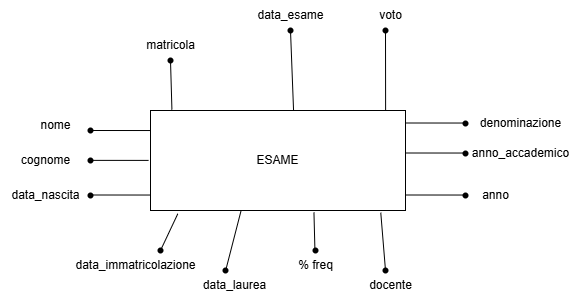
\includegraphics[width=1\textwidth]{images/EsercizioProgConc.png}
      \caption{esercizio}
  \end{figure}

  Questa soluzione presenta \textbf{diverse problematiche:}
  \begin{enumerate}
    \item  L'utente è legato all'esame, infatti un utente esiste solo se esiste anche un'esame. Per questo motivo sarebbe consono creare un'entità utente contenente nome, cognome, matricola...
    \item Cosa identifica nello specifica l'entità esame? Un appello? Un esame completo...?
    \item Dentro all'entitità dovrebbero esserci oggetti appartenneti ad un'unica classe (oggetti simili)
  \end{enumerate}
  
  Tutto questo porta a \textbf{rindondanza e ritardo nella memorizzazione dei dati.}

  Una possibile soluzione dell'esercizio è questa.
  \begin{figure}[h] %% Messo H anzichè h in questo modo il testo sotto non passa sopra la foto in quanto troppo grande
      \centering
      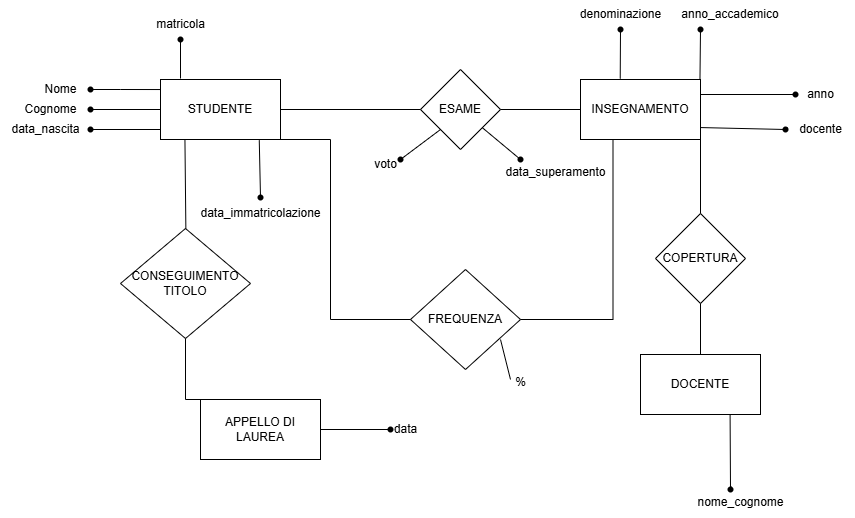
\includegraphics[width=1\textwidth]{images/ProgConcCorretta.drawio.png}
      \caption{esercizio}
  \end{figure}

  Come si può vedere, sono state create delle entità per studente e insegnamento. L'esame è diventato una relazione che lega lo studente all'insegnamento, cosi come lo è diventata la frequenza.
  
  
  \subsection*{Esercizio 2}
  \addcontentsline{toc}{subsection}{Esercizio 2}

  \esercizioTesto{Base di dati di una banca}{Si vuole progettare la basi di dati di una banca. La banca è suddivisa in filiali e di ogni filiale si conosce il nome, il codice numerico (univoco), l'indirizzo e il numero di clienti.
  
  I clienti della banca sono memorizzati nella base di dati. Per ogni cliente sono memorizzati: il nome, il cognome, il codice fiscale, la data di nascita e la professione. 
  
  La base di dati contiene inoltre i dati sui conti correnti aperti presso le filiali della banca. Ogni conto corrente viene aperto presso una e una sola filiale e ha una numerazione univoca nella filiale. Ogni cliente può aprire più conti (anche presso la stessa filiale) e un conto può avere più intestatari. 
  
  Si vuole mantenere traccia nella base di dati di tutte le operazioni (movimenti) eseguite sui conti correnti, indicando per ogni movimento, un numero progressivo univoco per conto corrente, la data, il tipo di operazione e il valore.

  Per ogni conto corrente si deve produrre il saldo. Si supponga che un cliente possa aprire conti diversi in più filiali della banca.}

  \begin{tikzpicture}[
  entity/.style={rectangle, draw=blue!50!black, thick, minimum width=3.2cm, minimum height=1cm},
  relationship/.style={diamond, draw=blue!50!black, thick, aspect=2, inner sep=1pt},
  attribute/.style={ellipse, draw=blue!50!black, thick},
  line/.style={draw=blue!50!black, thick},
  every node/.style={font=\sffamily}
]

% === NODI ENTITÀ ===
\node[entity] (filiale) {FILIALE};
\node[entity, right=6cm of filiale] (cliente) {CLIENTE};
\node[entity, below=3cm of $(filiale)!0.5!(cliente)$] (conto) {CONTO CORRENTE};

% === RELAZIONI ===
\node[relationship, below=of filiale] (gestisce) {gestisce};
\node[relationship, below=of cliente] (possiede) {possiede};

% === COLLEGAMENTI ===
\draw[line] (filiale) -- node[left]{(0,N)} (gestisce);
\draw[line] (gestisce) -- node[below]{(1,1)} (conto);

\draw[line] (cliente) -- node[right]{(1,N)} (possiede);
\draw[line] (possiede) -- node[below]{(1,N)} (conto);

% === ATTRIBUTI FILIALE ===
\node[attribute, above left=0.5cm and 0.5cm of filiale] (nomeFiliale) {nome};
\node[attribute, above right=0.5cm and 0.5cm of filiale] (codiceFiliale) {codice};
\draw[line] (filiale) -- (nomeFiliale);
\draw[line] (filiale) -- (codiceFiliale);

% === ATTRIBUTI CLIENTE ===
\node[attribute, above left=0.5cm and 0.5cm of cliente] (nomeCliente) {nome};
\node[attribute, above right=0.5cm and 0.5cm of cliente] (professione) {professione};
\draw[line] (cliente) -- (nomeCliente);
\draw[line] (cliente) -- (professione);

% === ATTRIBUTI CONTO ===
\node[attribute, below=0.7cm of conto] (numero) {numero};
\draw[line] (conto) -- (numero);

\end{tikzpicture}

\end{document}